\chapter{Organization and project management}
In this chapter, we will study how the project was managed, and the different steps we had to take in order to achieve all our goals.

\section{Technologies and methods}
We saw this project as a way to enact modern software development techniques.
\subsection{Agile methodology}
Even if we didn't explicitely named it, the method used was clearly agile, because every week or every two weeks we saw our clients and showed them our current progress, and we stated the goals for the following weeks.

\subsection{Softwares used}
We also used different software tools to manage the project.

\paragraph{Git and Github} 
They were used to hold the source files and the wiki. We also put our weekly reports here, which allowed the teachers to tell us what we had to improve. \brand{Git} is very useful for advanced softwares, even if we didn't use it to its maximum potential.
As well, we did not use every single feature of \brand{Github}, like bug reports.

\paragraph{Travis CI} 
A big advantage of Github is that it allows continuous integration with other services. We used \brand{Travis CI}. The idea is simple : everytime somebody does a commit, a remote build system fetches it, and tries to build it and runs an user-specified script (in our case, unit tests). If the build fails, or if the software ends in an erroneous state like with a segmentation fault, we get an email, and we can access the build and execution log to see what failed.

This can be used as a testimony to check that the project correctly builds on a minimal system.

\paragraph{Doxygen} was used for the documentation. Mostly everything is documented, the library as well as the graphical interface.

\paragraph{QtCreator} was the chosen development environment. It has a tight integration with \brand{qmake} as a build system, hence the hard dependency on it (which is anyway included with \brand{Qt}, required for the user interface). 

\paragraph{Qt Test Framework}
This test frameworkwas used for the unit test, in order to provide an easy-to-read output. It can also provide an Xunit XML output which is a standard unit test output, but we did not feel the need for it. 

\paragraph{cppcheck}
It is a static code analysis software which finds bugs unlikely to be found by a compiler, like memory leaks, array bounds overflow... We ran it regularly to check for potential bugs.

\paragraph{valgrind}
A big emphasis was put on the memory cleanliness : as a matter of fact, there is not a single memory leak in the library.

\paragraph{gcov}
This software was used to test the code coverage of the library during the unit tests, to ensure maximum efficiency for the other tools that we explained before.

\section{Schedule}
We will see here the repartition of the work on the project.

An important thing to keep in mind is that the project used an existing framework, which had some bugs : this helped to alleviate much of the required work.

\subsection{Work repartition}
The repartition was as follows : 
\begin{figure}[h!]
\centering
\begin{tabular}{|c|l|}
\hline
Person & Work done \\
\hline
Jean-Michaël Celerier & Work on the framework \\
Abdelhamid Cherif & Evaluation \\
Augustin Chevrier & Compression-expansion method \\
Alban De Martin & \ac{GUI} \\
Quentin Midy & \ac{LSB} Methods \\
Valentin Sarthou & \ac{SSW} Methods \\
Marc Queiros Soares & Compression-expansion method \\
\hline
\end{tabular}
\end{figure}

\subsection{Gantt Diagram}
A Gantt diagram was made to have an assessment and a track to follow. It is viewable on the next page.

\begin{sidewaysfigure}[h!]
\centering
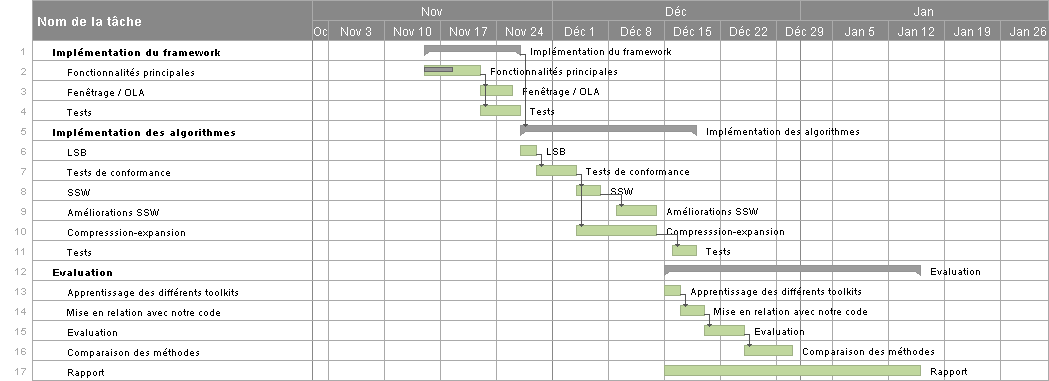
\includegraphics[scale=0.65]{images/gantt.png}
\caption{Approximative Gantt diagram for the project}
\label{gantt}
\end{sidewaysfigure}
